\documentclass[12pt]{article}
\usepackage[utf8x]{inputenc}
\usepackage{graphicx}
\usepackage{natbib}
\usepackage[left=1in, right=1in, top=1in, bottom=1in]{geometry}
\usepackage{titling}


\pretitle{\begin{center}\Huge\bfseries}
\posttitle{\par\end{center}\vskip 0.5em}
\preauthor{\begin{center}\Large\ttfamily}
\postauthor{\end{center}}
\predate{\par\large\centering}
\postdate{\par}

\title{SVHN: Machine Learning and Practical Image Recognition}
\author{Sajith Kumar (svaz0513), Sahar Nourazar (snou3270), James Macdonald (jmac7228)}
\date{\today}
\begin{document}

\maketitle
\thispagestyle{empty}

\begin{abstract}
This paper compares the performance of different machine learning algorithms on the Street View House Numbers dataset. This paper examines Support Vector Machines, Random Forest, and Neural Network methods, evaluating performance across a number of metrics.
\end{abstract}

\section{Introduction}
 
Machine learning has demonstrated reliable, accurate performance in image recognition tasks. On datasets such as MNIST, simple neural networks can achieve over 99\% accuracy \citep{tfmnist}. High performance is being achieved in other, more practical problems. The Street View House Numbers dataset (SVHN) is a series of labelled images depicting house numbers taken from google images. The dataset has been cropped to centre the relevant number in a 1024 pixel square image. The training set comprises 73,257 and the validation set contains a further 26,032 images. Training is conducted via cross-validation, but performance is determined by the accuracy achieved both on the kfold hold-out and the separate, hold-out validation set. Supplementary metrics will be similarly explored in further analysis.\\

The purpose of this study is twofold: firstly, to compare the performance of newer, specialist methods of image classification against that of more generalist algorithms. The generalist algorithms used are Support Vector Machines (SVM) and Random Forest (RF), and are 'generalist' in the sense that they have no special image recognition preprocessing. The specialist method is a Convolutional Neural Network (CNN), with two permutations. The first involves 'vanilla' CNN that stacks convolutional layers and fully-connected layers. The second permutation first uses a K-means clustering implementation to construct features, and feeds those features to a CNN for enhanced performance. This study will investigate the performance uplift of specialist methods over generalist methods.\\

The second purpose of this study is to investigate the 'accessibility' of top-of-the-range performance. The highest-scoring algorithms can achieve over 98\% out-of-sample accuracy. This study investigates how achievable those results for masters-level students with standard tooling and resources. For neural networks, this means a readily available solution like Tensorflow or Keras. For other classifiers, this means it must be available in the python data science library Scikit-Learn. Any preprocessing was done either using these or lower-level libraries, such as numpy.\\

This study is important because it draws a link between the cutting edge of machine learning techniques and mainstream implementations. It is important to democratize and propagate breakthroughs in academic research, and this study examines how far behind mainstream implementations lie.\\

\section{Methodology}

\subsection{The Problem}
The SVHN problem is similar to MNIST, in that the goal is to identify digits in images. However, the SVHN data adds a number of layers of complexity to the problem not present in MNIST. For one, SVHN contains data from real-world images, so there are complications such as lighting, rotation, viewing angle, and possible obstruction. Secondly, a given SVHN data may contain multiple numbers in a single frame, and the classifier must identify which ones are noise, and which ones are the label.\\

The classes are skewed, with certain numbers appearing much more frequently than others. This is to be expected, since the real-world prevalence of digits such as 1 would be much higher in the housenumbers scenario, as opposed to a digit like zero. This aspect of the data adds a further layer of complexity. The distribution of classes is shown below.\\
\begin{figure}[h]
\caption{Class distribution in the SVHN dataset}
\centering
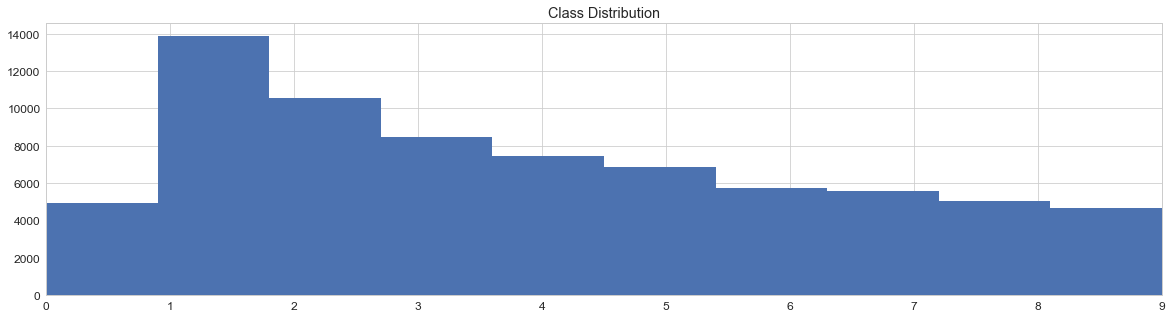
\includegraphics[width=0.9\textwidth]{images/svhn_classes.png}
\end{figure}


There is an additional, optional layer of difficulty in this problem. The SVHN data is presented in two forms, firstly the raw, unzoomed snapshots from Google Street View, secondly a tightly cropped set of 32x32 images that centre the relevant number. The first form of the data is a much trickier problem in that a classifier must first preprocess the image to detect an unknown number of numbers with unknown positions. This additional layer will not be looked at in the model comparison, but touched on in further analysis.\\

\subsection{Data Preprocessing}
As outlined in the introduction, this study compares 2 main types of approaches: generalist methods and specialist methods.\\

Firstly, the data is converted to greyscale. This significantly reduces the dimensionality of the data and thus makes training much faster. Colour plays no part in determining a number, so the conversion should not remove any useful information. The conversion to greyscale is done line with human sight, so channels are not uniformly weighted. Exact weights are given in the code.\\
\begin{figure}[h]
\caption{The effect of preprocessing the data from colour to greyscale}
\centering
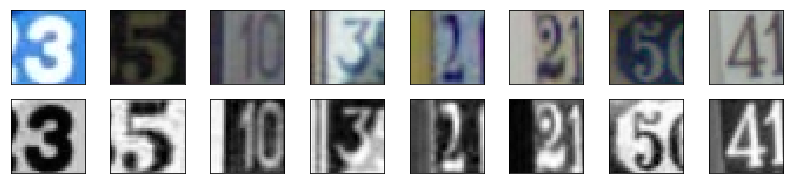
\includegraphics[width=0.9\textwidth]{images/colour_to_greyscale.png}
\end{figure}

Secondly, the data is run through a Principle Component Analysis (PCA). Reducing the dimensionality again allows for much faster training of the algorithm. However, since convolutional steps require the concept of the image in order to extract features, PCA was only done for generalist solutions.\\
\begin{figure}[h]
\caption{Information retained by taking the N largest eigenvalues}
\centering
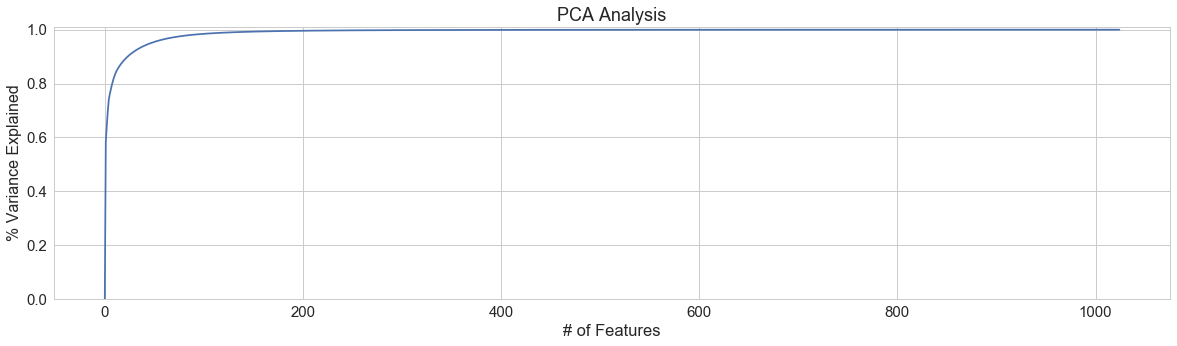
\includegraphics[width=0.9\textwidth]{images/pca_information_retention.png}
\end{figure}

\subsection{Generalist Solutions: Support Vector Machines}
The first classification approach used an SVM classifier on preprocessed data. SVM was chosen because it has previously seen considerable success in image-recognition problems \citep{svmkernels}.\\

Scikit-learn offers an out-of-the-box SVM classification tool, called SVC. There is some hyper-parameter tuning involved in fitting an SVC. For kernel selection, Gaussian methods outperform other variations for image classification\citep{svmkernels}, and for this reason the Gaussian Radial Basis Function (RBF) was selected. A Randomized Search was conducted on a 5000-row sample of the data to select the regularization parameter C, and the kernel coefficient gamma. Randomized search was chosen because it retains many benefits of Grid Search (simplicity in concept and implementation) while having high efficiency in high-dimensional search spaces. This hyperparameter tuning ran in just under 3 minutes.\\

After hyperparameter tuning, the algorithm was trained via k-fold cross validation with 10 folds. The holdout sets were scored, and those scores were combined to create the final scored dataset. The total 10-fold loop of the data took 93 minutes.\\

Unfortunately, SVM solutions do not neatly return the probabilities that each observation belongs to a given class. Scikit-learn's solution offers a heuristic but using this would have blown out training times by a factor of ten, making the algorithm unfeasible. As such, not all metrics could be calculated for the SVM solution.\\


\subsection{Generalist Solutions: Random Forest}
The second classification approach used a Random Forest (RF) algorithm. RF models are an ensemble of decision trees, which separate the data by splitting on features which best segment out distinct classes. Each tree is only exposed to a subset of features, which is chosen at random \citep{rfimages}. This structure means that the model automatically regularizes well, since no tree has the opportunity to learn the data. Additionally, the non-linearity of RF models mean that they can capture effects that are hidden from linear models, such as by splitting more than once on a given feature, and also automatically include cross-product effects. \\

The RF model was exposed to data that had been preprocessed firstly via greyscale and secondly with PCA to reduce the dimensionality and extract key features. This was possible because, like SVMs and unlike CNNs, RF models don't depend on a 2D image construct.\\

RF models have some hyperparameters that require tuning, namely max tree depth and total number of trees. These were tuned on a small, 2000-row sample of the data. Even though this subset was small, the evaluation of hyperparameters still took a very long time, running for 32 minutes. The results of the search are displayed in figure 4.  Due to the highly imbalanced classes, the class\_weight parameter was set to 'balanced', forcing the algorithm to draw class weights from the data. This was a good solution because the distribution of the test data matches the distribution of training data in K-fold due to the shuffling of the data.
\\
\begin{figure}[h]
\caption{Random Forest performance against tree count and depth: Darker is better}
\centering
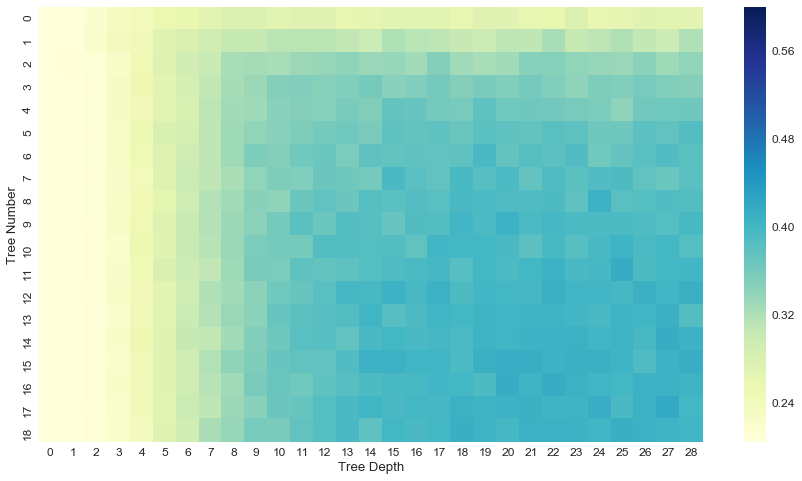
\includegraphics[width=0.9\textwidth]{images/random_forest_hyperparams.png}
\end{figure}


Once optimal values of hyperparameters were determined, the algorithm was trained via 10-fold cross validation, with hold-out sets combined into the results dataset. Training occurred remarkably quickly, with only 15 minutes required to complete all 10 folds. Furthermore, the RF solution allowed not only for the predictions but the model's estimated probability of each class.

\subsection{Specialist Solutions: Convolution Neural Network}
The final classification approach was a Convolutional Neural Network (CNN), a machine-learning algorithm adapted specifically for image classification tasks. CNNs consist of a number of trainable layers that fall into the following categories:\\
\begin{itemize}
  \item Convolutional layers: 2-dimensional filters applied to a subset of pixels that multiply the pixel fill by trainable weights
  \item Pooling layers: 2-dimensional filters that apply an operation over a subest of pixels, usually to extract the maximum value (a process known as maxpooling)
  \item Fully-Connected layers: A 1-dimensional array of trainable weights that multiply input features, and then apply a non-linear activation function (such as Rectified Linear Units)
\end{itemize}

There are two important attributes of CNNs that suit image recognition data. The first is the previously mentioned specialized layers (convolutional and pooling). Also, image data represents high-dimensional space. The training algorithms of neural networks scale much better than techniques like SVM, both in terms of dimensionality and number of observations.\\

In order to generalise the solution, both drop-out and l2 regularization techniques were employed. Drop-out prevents the network from leaning too heavily on individual nodes by assigning each node a probability that its output will be set to zero. L2 regularization applies a penalty to the magnitude of weights, encouraging the network to use smaller coefficients and thus inhibiting overfitting.\\

The full set of hyperparameters to be tuned in the neural network is:
\begin{itemize}
\item Batch size - how many observations exposed to the network at each iteration
\item Network architecture - such as  number of layers, type of layer, filters/neurons per layer
\item Dropout - the probability that a given node be switched off in training
\item L2 regularization - the strength of the penalty applied to coefficients
\item Learning rate - the rate of gradient descent the network employs
\item Number of iterations - how many batches the network will see in training
\end{itemize}

Unfortunately, there is no easy solution to the general problem of tuning Neural Network hyperparameters, as the search space is high-dimensional and also not continuous. Initial estimates were based on a mixture of sensible estimates and literature \citep{nnoptim}. Hences, these were all adjusted manually by observing network performance on out-of-sample data as hyperparameters were tweaked. This was sense-checked by confirming that out-of-sample performance reflected in-sample checks. \\

After tuning, a K-fold cross validation was performed on the training dataset. While K-fold is not usually done with neural networks \citep{nnoptim}, it was done in order to keep results comparable to the other algorithms. The in-sample performance was tracked to see the performance of the AdamOptimizer algorithm. This is shown in figure 5:\\

\begin{figure}[h]
\caption{CNN in-sample performance by iteration (the average is given in black)}
\centering
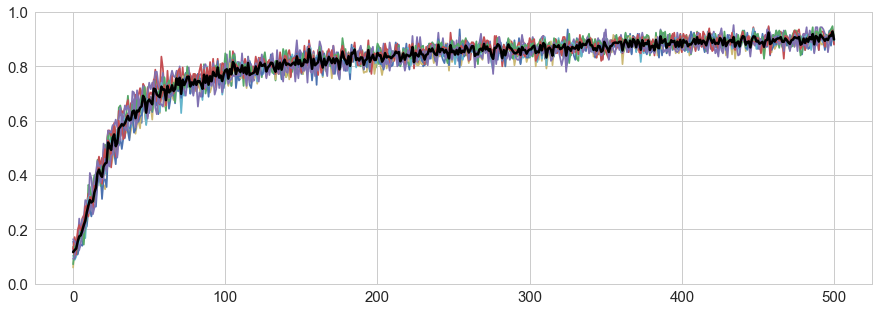
\includegraphics[width=0.9\textwidth]{images/training-progress.png}
\end{figure}

Running the optimization further did not improve out-of-sample performance, and increased an already-substantial training time.

\section{Experiments and Discussion}
\subsection{Results and Comparison}

The accuracy achieved in the K-fold cross validation exercise was 64.65\% for RF, 79.54\% for SVM and 85.62\% for CNN. A full breakdown of results achieved by each algorithm is given in the table below:\\
\begin{center}
\begin{tabular}{ c c c c c }
 Algorithm & Precision & Recall & F1 Score & Accuracy\\ 
 RF & 0.68 & 0.64 & 0.63 & 0.64 \\  
SVM & 0.80 & 0.80 & 0.79 & 0.80\\
CNN & 0.86 & 0.86 & 0.86 & 0.86                    
\end{tabular}
\end{center}

These results were expected, and are in line with the optimization of each algorithm to the problem.They also reflect the time taken to achieve these results. The RF model was surprisingly quick to train, with all folds completed in 15 minutes. SVM took much longer, at 93 minutes, and CNN took the longest at 210 minutes.\\

These results neatly illustrate the resource cost of performance as more sophisticated techniques are implemented. However, if the dataset were to increase, this relationship might not hold. The cost of training an SVM model increases exponentially with the data at $O(n^2)$ when the cost of errors is small, and $O(n^3)$ when cost of errors is large \citep{algoperformance}. By contrast, neural networks scale linearly due to the batching technique. While the SVM model trained quicker than the CNN, this might not reflect performance on larger datasets.\\

The confusion matrix of each classifier shows its strengths and weaknesses when it deals with particular classes. The values of the squares are out of a total of 100\%, determined what share of the label's prevalence (not prediction) is in that square.\\
\begin{figure}[h]
\caption{The Confusion Matrix for each classifier}
\centering
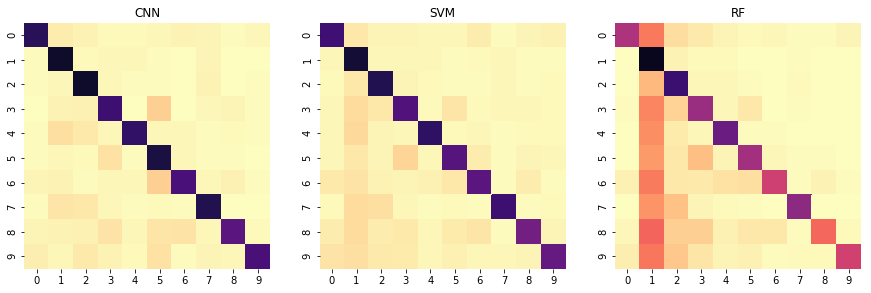
\includegraphics[width=0.9\textwidth]{images/cm_all.png}
\end{figure}

The confusion matrices are in sync with the accuracy results outlined previously. CNN has a marginally better confusion matrix than SVM, while RF lags behind both. Interestingly, it looks as though a lot of RF's error comes from the balance issues in the dataset. The overrepresentation of '1' in the data has hampered the precision on that class but greatly increased the recall. This comes at the cost of recall for other classes. This is despite the setting of the class\_weight hyperparameter to 'balanced', and might suggest that hyperparameter is not sufficiently accounting for class imbalance.\\

From this analysis, it is clear that CNN is the best classifier for this problem, followed by SVM and RF.\\

\subsection{Additional Metrics}

Another powerful metric for examining model performance is the ROC AUC curve. Unfortunately, as previously outlined, the SVM algorithm does not naturally compute probabilities, and Scikit-learn's heuristic would have been too computationally expensive for a feasible solution. As a result, only RF and CNN can be compared. The results are still worth examining.\\

The ROC AUC score provides a number out of 100\% that indicates how well a classifier ranks predictions. It can be generalised to multiclass problems by weighting on class prevalence. The ROC results for RF and CNN are shown below. Not surprisingly, the CNN greatly outperforms the RF classifier, at 96.83\% to 91.48\%.\\

However, the RF ROC curve looks particularly impressive for a classifier that only scored 64\% accuracy. The reason for this is twofold. Firstly, the ROC curve really only plays in the space above the 45-degree line. Anything below that line performs worse than random chance, so it acts as a baseline for model performance. A naive estimator that selects '1' for every observation would achieve 18.9\ accuracy, while the RF classifier achieves 64\%. Secondly, ROC curves reward classifiers that assign high probabilities to the correct class even if that class did not receive the maximum probability.The RF classifier might be assigning a high second probability to the correct class, giving it better performance in the ROC AUC metric

\begin{figure}[h]
\caption{The ROC Curves for RF and CNN Classifiers} 
\centering
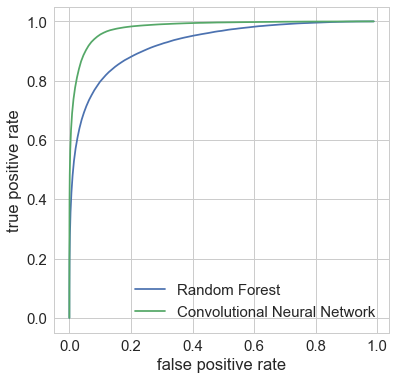
\includegraphics[width=0.5\textwidth]{images/roc_curves.png}
\end{figure}



\subsection{Wider Comparison}

The findings in the above section correspond with the literature on this problem. The top-performing models on the SVHN dataset are predominantly Convolutional Neural Networks \citep{problemperformance}. Furthermore, Deep Learning implementations dominate the leaderboards of MNIST, CIFAR-10, CIFAR-100 and STL-10 classification problems.\\

However, despite this finding, this study was unable to replicate the success of the above neural networks. On the SVHN dataset, top-tier solutions can achieve an out-of-sample error of under 2\% \citep{problemperformance}, a factor of ten better than this study's best model. This could not be achieved by our solution without blowing out the number of layers and parameters. For example, the top-performing network found has convolution layers of 128, 128, 320, 320, 384 and 384 channels, and pooling layers of 96, 256, 256 channels \citep{bestsvhn}. In contrast, this study uses a network of 16,32,64,128 convolutional layers with pooling occurring within those layers. The additional complexity of the cited solution would have increased training times to unacceptable levels.

\subsection{Image Detection and Classification}

Everything discussed so far only relates to the simplest problem of single-digit recognition. There was some brief exploration of a more difficult problem, classifying multiple digits per image. This additional exercise was performed using a convolutional neural network similar to the above, but with feature preprocessing performed by a K-means clustering step. This technique was adopted from the paper, 'Convolutional Neural Networks Embedding K-means' \citep{kmeanscnn}. The clustering step produced well-behaved features that were then fed to a neural network. However, instead of taking the argmax of the softmax output to determine a sole class, multiple classes were kept in the output and all classes that met the probability threshold were given as predicted.\\

This classifier performed very well, and achieved a validation accuracy of 87.91\%. However, since it was answering a fundamentally different problem to the previous, this result cannot be compared to the other methods.\\


\section{Conclusion}

It is true that once trained, scoring a neural network is relatively trivial. However, replicating the creation of remarkable neural networks is dependent on one's access to similarly remarkable computing resources. The conclusion of this observation is that while academia has made great strides in the image classification field, the capabilities unlocked are only at the disposal of entities with significant resources at their disposal.\\

This study leads naturally to some next steps. There are important aspects of the SVHN problem that have been simplified away in this study. Specifically, in the original raw images, the locations of numbers are given by coordinates in the metadata. It would be a good next step to train a model to detect the presence of numbers in an image, and then feed cropped images to another classifier such as the ones implemented in this study. This would be a significant step in bringing such classifiers into more practical use, since it is rare to get neatly defined images that centre the object of interest, especially in situations such as house number recognition.

\medskip
 
% To change the title from References to Bibliography:
\renewcommand\refname{Bibliography}

\bibliographystyle{unsrtnat} % or try abbrvnat or unsrtnat
\bibliography{references} % refers to example.bib
 
\end{document}
